\chapter{使用特权信息学习范式的无人机集群行为分类研究}
\label{chap:intelligent-learning}

\section{引言}
自Vapnik和Chervonenkis提出模式识别理论后\citep{vapnik1974}, 强机器学习理论的知识已经被建立起来 \citep{vapnik1974,vapnik1979,vapnik1982,vapnik1995,vapnik1998,Vapnik2006,Chervonenkis2013}。第\ref{chap:edbed}章给出的也是强机器学习理论一致收敛的充分必要条件, 根据第\ref{chap:edbed}章的研究内容, 强机器学习理论已经解决如下关于机器学习的基础问题:
\begin{enumerate}
\item 学习过程收敛的充分必要条件(第\ref{sec:uniform-convergence}节给出),
\item 学习过程收敛的速度的界(第\ref{sec:rate-of-convergence}节给出),
\item 基于容量控制的一种新归纳推理原则——结构风险最小化原则——通过控制两个因素(即最小化经验风险泛函和容量)使得学习模型总是收敛至最优的逼近函数(第\ref{sec:special-case}给出),
\item 开发的SVMs算法实现结构风险最小化原则。
\end{enumerate}

因此关于一般学习理论的研究似乎完成: 因为以上四个问题几乎在理论上完整回答所有与统计推理相关的问题, 剩下的只是一些修修补补。 例如用第\ref{chap:Swarm-MCP}章提出的一致性预测为机器学习算法输出给出一些可信程度的度量; 用第\ref{chapter:swarm-distributions}章介绍的无分布假设的鞅方法提供分布漂移检测并且当发生分布漂移时重新训练模型即可; 或者根据第\ref{chapter:swarm-martingales}章介绍的鞅保护分布方法提升机器学习的预测能力。虽然上述章节提出的方法在一定程度上能够提供一些改进, 但是确切说来这些改进都建立在第\ref{chap:edbed}章的研究内容之上。所以从理论层面而言, 似乎的确关于一般学习理论的研究已然完成。

然而, 核心问题总藏在理论阐述的细节之处\citep{Vapnik-similary-2015,Vapnik2021}。通过对比人类学习和机器学习之后就不难发现, 人类学习所需要的样本要比机器学习少得多。在前面章节的模型构建中, 大都需要上千个训练样本才能得到相对令人满意的结果, 但是显然对于人类而言并不需要太多的样本就可以完成相当不错的学习。从提供学习一致性收敛的VC理论来看, 第\ref{chap:edbed}章的研究已经表明, 学习一致收敛依赖于两个因素: 即一方面取决于分类规则将下列训练数据分开的质量
\begin{align}
\label{ch4:train-data}
(x_{1}, y_{1}), \ldots, (x_{l}, y_{l}), x \in R^{n}, y \in \{-1, +1\},
\end{align}
另一方面取决于被选中的规则所在的诸函数的集合本身的VC维。

形式化而言, VC理论有两种明显不同的情形:
\begin{enumerate}
\item[1.] \textsf{对于可分情形:} 根据第\ref{chap:edbed}章中第\ref{sec:kefen}节的内容, 这种情形下在具有有限VC维$h$的诸函数$f(x,\alpha), \alpha \in \Lambda$的集合中, 存在一个函数$f(x,\alpha_{l})$其能够将训练数据 (\ref{ch4:train-data})完全正确地分开, 即
\begin{align}
y_{i}f(x_{i}, \alpha_{l}) > 0, \forall i = 1, \ldots, l.
\end{align}
在这种可分情形下, 一致收敛的速度的界
\begin{align}
P(yf(x, \alpha_{l}) \leq 0) < O^{*}\left(\frac{h - \ln \eta}{l}\right)
\end{align}
以概率 (with probability) $1-\eta$ 成立。 其中, 这里$P(yf(x, \alpha_{l}) \leq 0)$是函数$f(x, \alpha_{l})$错误分类的概率, $h$是诸函数可行集的VC维, 标识符$O^{*}$表示的是对数因子高阶项的阶数。
\item[2.] \textsf{对于不可分情形:} 根据第\ref{chap:edbed}章中第\ref{sec:special-case}节的内容, 这种情形下在具有有限VC维$h$的诸函数$f(x,\alpha), \alpha \in \Lambda$的集合中, 不存在函数能够将训练数据 (\ref{ch4:train-data})完全正确地分开。 因此, 设$f(x, \alpha_{l})$是在训练集(\ref{ch4:train-data})上最小化分类错误数目的函数, 令$v(\alpha_{l})$是此函数在训练集上的错误频率。那么根据VC理论, 下列一致收敛的速度的界
\begin{align}
P(yf(x, \alpha_{l}) \leq 0) < v(\alpha_{l}) + O^{*}\left(\sqrt{\frac{h - \ln \eta}{l}}\right)
\end{align}
以概率 (with probability) $1-\eta$ 成立。
\end{enumerate}

也就是说, 在可分情形下一致收敛的速度的界具有$O(\frac{1}{l})$的阶数; 而在不可分情形下一致收敛的速度的界具有$O(\frac{1}{\sqrt{l}})$的阶数。 换言之, 这表明为获得相同阶数的收敛, 在可分情形下只要$100$个样本而在不可分情形下则需要$100^{2} = 10000$个样本。 

为什么根据VC理论, 可分情形和不可分情形需要的样本数目会产生如此这般巨大的差别, 这种差别正就类似于人类学习和机器学习之间的差别。Vapnik认为人类学习和机器学习之间产生差距的原因在于“人类实现快速学习的原因是因为人类有老师的指导”\citep{vapnikinterview2014,vapniktalk2022,vapniktalk2022-02}, 能够在VC维对知识本身展开学习\citep{Vapnik-rethinking-2018,vapnik2020,Vapnik2021,2019Reconciling}。 使用特权信息学习 (Learning Using Privileged Information, LUPI)\citep{Vapnik2009,vapnik2015}模型基于这一思想出发, 可以提供在小样本下实现高精度的学习范式。

本章首先介绍LUPI方法的相关研究, 然后基于LUPI方法提出使用整体描述信息作为特权信息加速学习算法的收敛速度, 构建在两种不同类型的整体描述信息下无人机集群行为分类的LUPI学习范式, 进而将提出的方法应用于三种公开无人机集群行为数据集。最后, 通过数值算例对所提方法的可行性和有效性进行验证。


\section{使用特权信息学习方法的理论研究}
本节首先解释为什么在可分情形和不可分情形下学习算法的收敛速度会产生如此大的差距。

利用SVMs来说明这一问题。SVMs首先将空间$X$的向量$x$映射至空间$Z$中的向量$z$, 然后在空间$Z$构建分隔超平面。 对于可分情形, SVMs最小化下列泛函
\begin{align}
\mathcal{T}(w) = (w, w)
\end{align}
其约束条件是
\begin{align}
(y_{i}((w, z_{i}) + b)) \geq 1, \forall i = 1, \ldots, l;
\end{align}
而对于不可分情形, SVMs最小化下列泛函
\begin{align}
\mathcal{T}(w) = (w, w) + C\sum_{i=1}^{l}\xi_{i}
\end{align}
其约束条件是
\begin{align}
(y_{i}((w, z_{i}) + b)) \geq 1 - \xi_{i}, \forall i = 1, \ldots, l;
\end{align}
其中, 这里的$\xi_{i} \geq 0$ 都是松弛变量。 这就是说, 在可分情形下SVMs使用$l$个样本估计向量$w$的$N$个系数; 而在不可分情形下SVMs使用$l$个样本估计$N+l$个系数——向量$w$的$N$个系数和松弛变量$\xi_{i}$的$l$个取值。 因此, 在不可分情形下需要估计的参数个数$N+l$始终大于样本数$l$。 因为松弛变量大多取值为0并不会影响这种局面, 所以可能是SVMs需要估计的参数个数造成这种差距。

现在考虑伴随神谕老师(Oracle Teacher)的SVMs。 假设老师能先入之见地提供给学生诸松弛变量取值(将这些“先入之见的信息”称为“特权信息”\citep{Husser1928,Husser1948-en}), 那么在训练阶段, 就可以拥有下列三元组数据
\begin{align}
(x_{1}, \xi_{1}^{0}, y_{1}), \ldots, (x_{l}, \xi_{l}^{0}, y_{l}),
\end{align}
其中, 这里$\xi_{i}^{0}, i = 1, \ldots, l$是所有贝叶斯决策规则的松弛变量。 因此, 为构建决策规则, SVMs必须最小化下列泛函
\begin{align}
\mathcal{T}(w) = (w, w)
\end{align}
其约束条件是
\begin{align}
y_{i}((w, z_{i}) + b) \geq r_{i}, \forall i = 1, \ldots, l,
\end{align}
其中, 这里
\begin{align}
r_{i} = 1 - \xi_{i}^{0}, \forall i = 1, \ldots, l.
\end{align}
因为有神谕老师能够提供贝叶斯决策规则的松弛变量, 原本不可分的问题转变为可分问题, 收敛速率就等于$O^{*}(\frac{1}{l})$。\citet{Vapnik2009}证明神谕老师范式下学习的收敛速率。
\begin{proposition}\citep{Vapnik2009}
设$f(x, \alpha_{0})$是来自于VC维为h的诸示性函数$f(x,\alpha), \alpha \in \Lambda$的集合的函数, 此函数能够最小化分类错误的频率, 令
\begin{align}
\xi_{i}^{0} = \max \{0, 1-f(x_{i}, \alpha_{0})\}, \forall i = 1, \ldots, l.
\end{align}
那么对于满足下列约束条件
\begin{align}
y_{i}f(x_{i}, \alpha_{l}) \geq 1 - \xi_{i}^{0}, \forall i = 1, \ldots, l
\end{align}
的函数$f(x, \alpha_{l})$的概率$p(\alpha_{l})$是以概率 (with probability) $1 - \eta$界住, 即
\begin{align}
p(\alpha_{l}) \leq P(1 - \xi^{0} < 0) + O^{*}\left( \frac{h - \ln \eta}{l}\right).
\end{align}
\end{proposition}

LUPI学习范式通过引进特权信息——这种信息只能够在训练阶段有用而无法在测试阶段使用——来加速学习问题的收敛速度。在近期研究中, \citet{Vapnik-similary-2015,vapnik2015}揭示通过知识转化可以得到LUPI的稳定求解, 这种方法将学习模型的输出作为特权信息。\citet{Shiao2014} 将LUPI学习范式应用于生存数据建模, 提出一种基于LUPI范式的生存数据模型, 根据LUPI学习范式可以方便地将统计学中难以处理的生存数据切分为常规输入和特权信息输入, 进而获得高效的求解。\citet{Vrigkas2017}基于LUPI范式开发出一种提供现代新型人机交互识类型的识别算法, 研究者可以提供丰富的特权信息以加速识别算法的收敛。\citet{Izmailov2017}则考虑将LUPI应用于特征选择问题中, 他们将只能在训练阶段可用而在测试阶段不可用的特征作为特权信息, 以此基于LUPI范式实现高效的特征选择。 \citet{Izmailov2018} 将LUPI特征选择方法改进为一种自动特征选择方法, 这种LUPI类型算法不仅能够实现特征选择自动化, 而且能够充分利用潜在数据扩大备选特征的规模, 进而提高整体模型的预测效果。

根据文献调研, 鲜有在无人机集群领域中关注到LUPI类型的学习范式, 提出将无人机集群数据中的整体描述信息作为特权信息, 并构建LUPI模型加速底层学习算法的收敛速度。

\section{无人机集群使用特权信息学习方案设计}
\label{sec:swarm-behavior-empirical}

对于无人机集群行为分类问题, 当前的研究大都将之归约为监督学习问题, 然后借用机器学习算法逼近最优函数。 例如\citet{Tunstrm2013} 指出通过使用排序后的参数集合可以描述集群的机动结构。 \citet{Michael2014} 则报告针对大规模仿真机器智能体的自组织系统, 其通过成百上千个智能体通过彼此之间的信息交互就可以形成高度复杂的集群行为。 \citet{Brown-Human-swarm2014} 使用高阶吸引子集群模型来管理集群系统的整体行为。\citet{Brown2014} 则给出一种用于集群分类的创新框架, 这种框架通过使用局部近似模型来区分两种仿生集群行为。 \citet{Walker2014}则利用高斯模型来重建集群行为模式, 特别地, 在这篇文章中作者是采用集群个体的速度场作为模型输入, 然后通过高斯过程模型来实现集群行为的分类。\citet{Berger2016} 提出一种压缩子空间方法求解集群行为分类。 他们将单个智能体的速度域数据作为模型输入, 通过借用SVMs将之映射至低维数空间来实现集群行为的分类。

所有这些已发表的文献其实都希望借用机器学习方法实现复杂集群行为的分类, 并且从理论上分析可知这些研究都可以被归约为模式识别问题来处理。 从形式上看可表述为给定下列数据对 
\begin{align}
(x_{1}, y_{1}), \ldots, (x_{l}, y_{l}), \quad x_{i} \in X, y_{i} \in \{-1, 1\},
\end{align}
假设这些数据对是根据某个固定的、但是未知的概率测度$P(x,y) = P(y|x)P(x)$生成的。 机器学习算法在给定的诸示性函数的集合$f(x,\alpha), \alpha \in \Lambda$——诸示性函数的集合是由机器实现的——中找一个函数$y = f(x, \alpha_{0})$, 此函数能够最小化错误分类的个数。 在无人机集群行为分类问题中, 这里的输入向量$x_{i} \in X$由位置域组成, 而$y_{i} \in \{-1, 1\}$就是无人机集群整体对应的标签。

然而, 在构建学习算法时不仅仅局限在上述已经给出的数据集, 研究者对数据集本身的直观描述也是可用的。 的确, 对于集群行为分类问题而言, 在训练阶段不仅仅位置域信息可用, 而且一些额外的信息也是可以获得的。 比如, 在训练阶段是能够获取智能体彼此之间的交互信息的, 但是这种交互信息仅仅在训练数据集上可以获得, 无法在测试数据集上使用。 因此, 考虑如何将这种额外信息与现有模型融合, 进而期待能够加速学习收敛速率。 形式化而言, 考虑使用LUPI范式来处理集群行为分类任务, 这种学习范式给定三元组数据集合
\begin{align}
(x_{1}, x_{1}^{*}, y_{1}), \ldots, (x_{l}, x_{l}^{*}, y_{l}), \quad x_{i} \in X, x_{i}^{*} \in X^{*}, y_{i} \in \{-1,1\},
\end{align}
此三元组数据是由固定的、但是未知的概率分布$P(x,x^{*},y) = P(y, x^{*} | x)P(x)$生成。 现在的问题是在给定的诸示性函数$f(x,\alpha), \alpha \in \Lambda$集合中——诸示性函数集合由机器实现——找到一个函数$y = f(x, \alpha_{0})$, 此函数能够最小化错误分类的数目。 在这个模型中, 假设向量$x_{i} \in X$是由某固定的、但是未知的概率分布$P(x)$生成, 输入变量不仅仅是无人机集群对应的标签$y_{i} \in \{-1, 1\}$, 同时也提供特权信息$x_{i}^{*} \in X^{*}$, 此特权信息服从未知的条件概率函数$P(y_{i},x_{i}^{*} | x_{i})$。 例如, 在集群行为分类问题中的特权信息$x_{i}^{*} \in X^{*}$可以是由人类提供的某种整体描述, 并且这种整体描述仅仅在训练阶段可用。


针对处理复杂无人机集群行为识别问题, 提出考虑将人机交互信息——即人对于输入数据的整体描述——通过LUPI范式实现知识转换。 引进两种类型的特权信息, 其一是对整个无人机集群的整体合作描述, 其二是智能体彼此之间的内在竞争信息。 

图 \ref{fig:demo}展示在无人机集群的整体合作描述下的LUPI学习范式。如图所示, 训练阶段的输入不仅仅包含常规位置域信息(分别展示Align行为, Torus行为和Random行为等), 而且还包括特权信息(这些特权信息分别表示为Align*, Torus*和Random*)。不同的集群行为对应不同的特权信息$X^{*}$。所有的特权信息仅仅在训练阶段可用, 在测试阶段无法使用。因此, 一旦LUPI模型训练完成, 在测试阶段仅将常规位置域信息输入LUPI模型来获得对应的预测结果。

\begin{figure*}
\centering
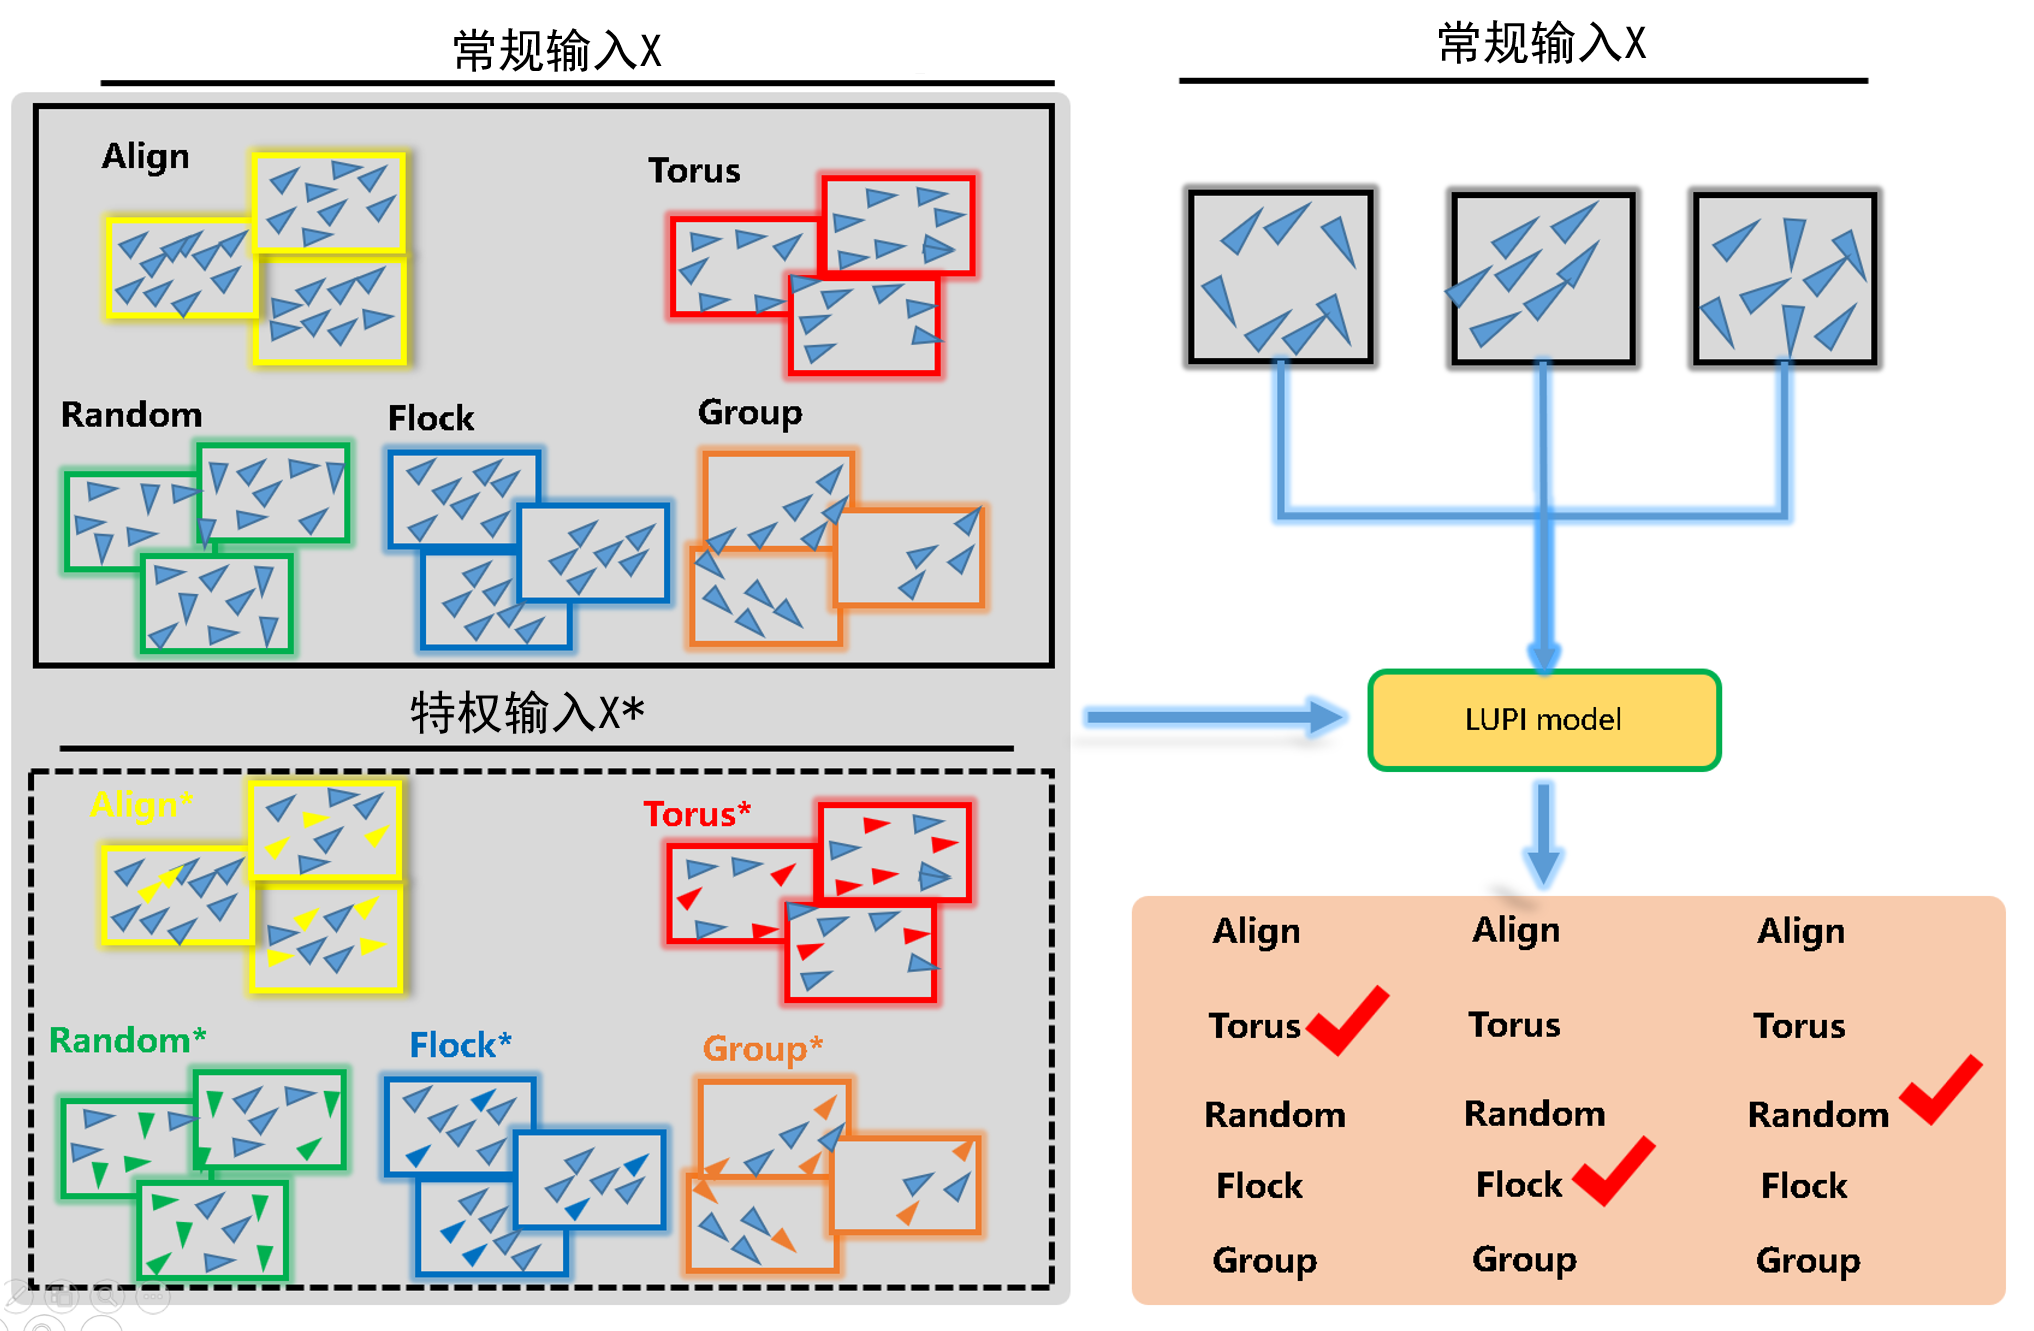
\includegraphics[width=1\textwidth]{Img/chapter10/LUPI.png}
\caption{使用特权信息学习范式方案设计框架图}
\label{fig:demo}
\end{figure*}

为学习所求的决策函数$y = f(x)$, LUPI方法首先将决策空间$X$中的向量$x$映射至特征空间$Z$中的向量$z$, 将特权空间$X^{*}$中的向量$x^{*}$映射至特征空间$Z^{*}$中的特征向量$z^{*}$, 在特征空间构建最优分隔超平面。 形式化的表述, 即考虑最小化下列泛函
\begin{align}
R(w, w^{*}, b, b^{*}) = \frac{1}{2}[(w, w) + \gamma (w^{*}, w^{*})] + C\sum_{i=1}^{l}[(w^{*}, z_{i}^{*}) + b^{*}]
\end{align}
其约束条件是
\begin{align}
&y_{i}[(w, z_{i}) + b] \geq 1 - [(w^{*}, z_{i}^{*}) + b^{*}], \quad i = 1, \ldots, l,\\
&[(w^{*}, z_{i}^{*}) + b^{*}] \geq 0, \quad i= 1, \ldots, l.
\end{align}

为求解此优化问题, 考虑其对应的Lagrangian乘子
\begin{equation}
\begin{aligned}
L(w, b, w^{*}, b^{*}, \alpha, \beta) &= \frac{1}{2}[(w, w) + \gamma (w^{*}, w^{*})] + C\sum_{i=1}^{l}[(w^{*}, z_{i}^{*}) + b^{*}]\\
& - \sum_{i=1}^{l}\alpha_{i}\left[y_{i}[(w, z_{i}) + b] - 1 + [(w^{*}, z_{i}^{*}) + b^{*}]\right]\\
& - \sum_{i=1}^{l}\beta_{i}\left[(w^{*}, z_{i}^{*}) + b^{*}\right]
\end{aligned}
\end{equation}
针对$w,b,w^{*},b^{*}$求此Lagrangian的最小化, 针对Lagrangian算子$\alpha \geq 0, \beta \geq 0$求此Lagrangian的最大化。

通过求解下列对偶问题可得LUPI问题的解, 即最大化下列泛函
\begin{equation}
\begin{aligned}
R(\alpha, \beta) &= \sum_{i=1}^{l}\alpha_{i} - \frac{1}{2}\sum_{i,j=1}^{l}\alpha_{i}\alpha_{j}y_{i}y_{j}(z_{i},z_{j})\\
& - \frac{1}{2\gamma}\sum_{i,j=1}^{l}(\alpha_{i} + \beta_{i} - C)(\alpha_{j} + \beta_{j} - C)(z_{i}^{*}, z_{j}^{*})
\end{aligned}
\end{equation}
其约束条件是
\begin{align}
&\sum_{i=1}^{l}(\alpha_{i} + \beta_{i} - C) = 0,\\
&\sum_{i=1}^{l}y_{i}\alpha_{i} = 0,\\
&\alpha_{i} \geq 0, \beta_{i} \geq 0, i = 1,\ldots,l.
\end{align}
其中, 这里 $(z_{i},z_{j}) = K(x_{i}, x_{j})$ 并且 $(z_{i}^{*}, z_{j}^{*}) = K^{*}(x_{i}^{*}, x_{j}^{*})$ 分别是在空间 $X$ 和空间 $X^{*}$上的核函数。

根据Vapnik-Chervonenkis理论\citep{Vapnik2006}, 此问题的解 $(w,b)$ 定义的分类超平面在\textsf{不可分情形}下的错误率\textsc{以概率} (with probability) $1-\eta$ 的界为
\begin{align}
P_{test} \leq v_{train} + O^{*}(\sqrt{\frac{VCdim}{l}}),
\end{align}
然而, 如果给定某三元组序列中的特权信息$x_{i}^{*}, i=1,\ldots,l$都是针对那最优超平面的理想变量 (ideal variables)的话——此时就将\textsf{不可分问题}转变为\textsf{可分问题}——那么此问题的解 $(w,b)$ 所定义的分类超平面的错误率就\textsc{以概率} (with probability) $1-\eta$被下列表达式界住
\begin{align}
P_{test} \leq v_{train} + O^{*}(\frac{VCdim}{l}).
\end{align}


采集的数据集仍然是根据公开发表在UC Irvine 机器学习数据仓库上的无人机集群行为数据集。 这一数据由澳大利亚新南威尔士大学托管的一个在线调查获得, 此数据包含三种行为数据集, 分别是\texttt{Flock}行为, \texttt{Align}行为和 \texttt{Group}行为。 在线调查的数据本身也是基于某无人机集群行为模型, 但是其标签是由参加在线调查的用户标记。 第\ref{chap:Swarm-MCP}章的表 \ref{tab:datainfo} 汇总介绍真实集群行为数据集的概要信息, 这些属性参见第\ref{chap:Swarm-MCP}章第\ref{sec:truth-swarm}节中的介绍。

现在介绍针对无人机集群行为识别如何在技术上落地LUPI学习范式。 无人机集群行为预测的核心问题是将无人机集群整体刻画作为特权信息, 本文拟提供两种整体性描述信息来加速计算机识别的收敛速度。在本文中所谓“加速学习收敛速度”, 并不是在更短时间计算出结果, 而是使用更少的样本使得学习算法收敛。 

将描述智能体之间的合作关系——即每个智能体的Alignment和Cohesion半径内智能体数目{nAC}——作为第一种整体性描述的特权信息。 根据\citet{Flocks1987}提出的“Boids”三原则理论, Alignment和Cohesion向量刻画的是智能体彼此之间处于聚集状态的向量, 因此, 在Alignment和Cohesion向量半径内的智能体数目直观上可以视为是一种合作关系的尺度。图 \ref{fig:nAC-demon} 展示两种集群类型下作为整体描述的特权信息{*nAC}的图示。 图\ref{group-sample5-coh} 展示的是Group行为, 此时其对应的特权信息{Group:*nAC}为图\ref{group-sample5-coh1}。 在特权信息{Group:*nAC}图中采用热力图标示{nAC}数目的大小。 从图中可以看到, 在智能体聚集的部分其特权信息{Group: *nAC}的取值也较高; 在智能体散开的部分其特权信息{Group: *nAC}的取值较低。因此, {nAC}数目的大小可视为智能体之间合作关系的一种度量。

%\begin{figure}
%\centering
%\includegraphics[width=.4\textwidth]{Img/chapter10/Class-group-sample5.pdf}
%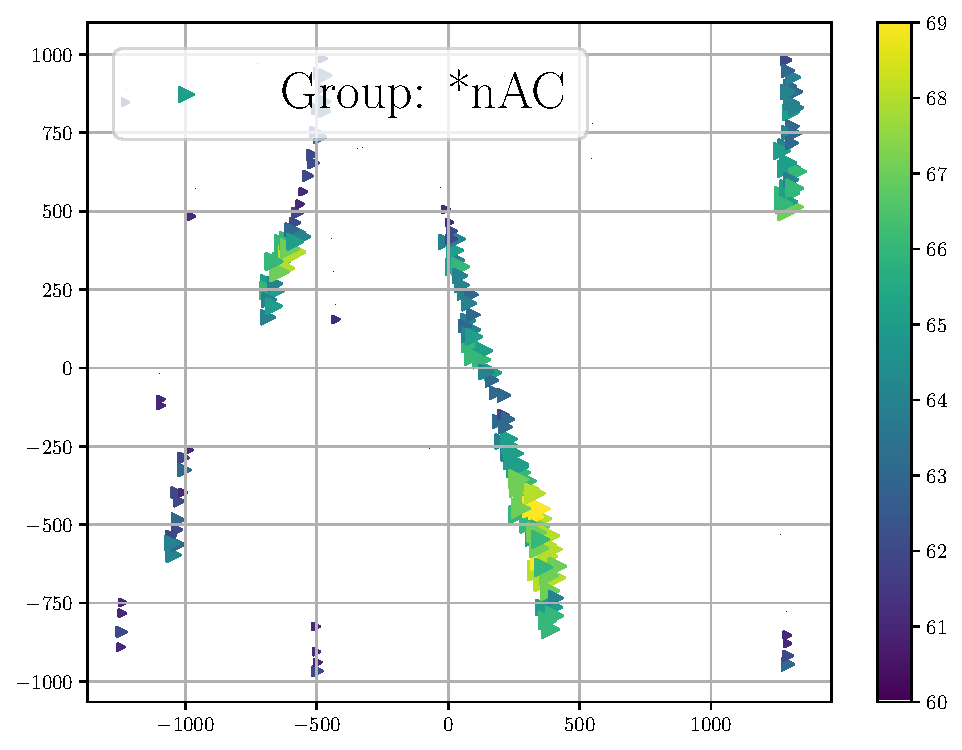
\includegraphics[width=.4\textwidth]{Img/chapter10/PI-Class-group-sample5.pdf}
%\includegraphics[width=.4\textwidth]{Img/chapter10/Class-align-sample4.pdf}
%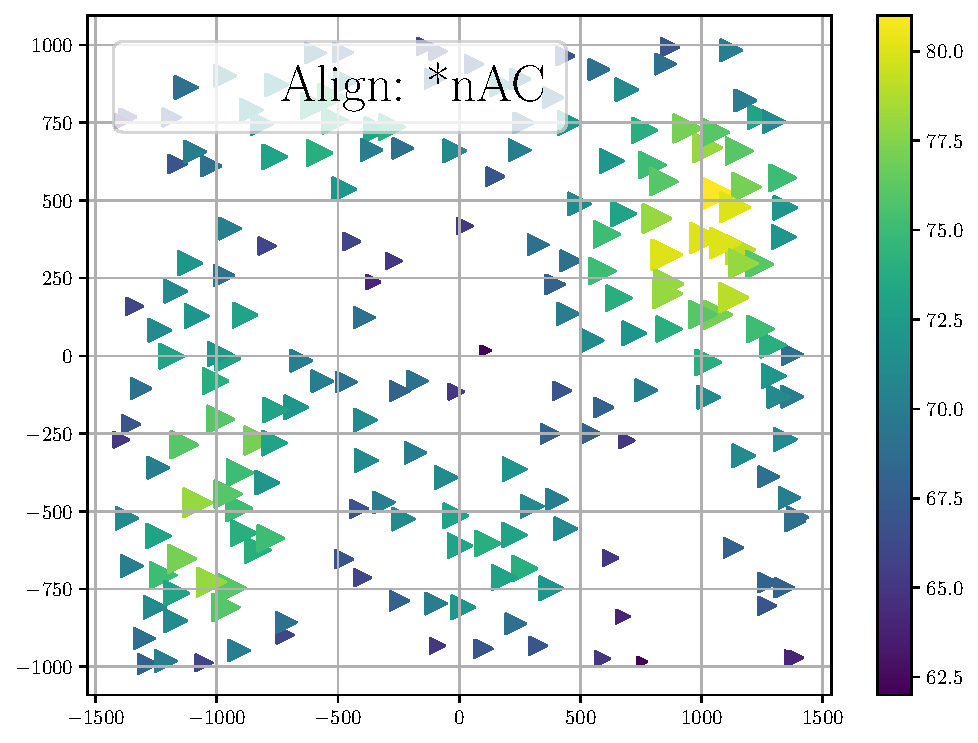
\includegraphics[width=.4\textwidth]{Img/chapter10/PI-Class-align-sample4.pdf}
%\caption{智能体合作关系的整体描述示意图}
%\label{fig:nAC-demon}
%\end{figure}

\begin{figure}
     \centering
     \begin{subfigure}[b]{.45\textwidth}
         \centering
         \includegraphics[width=1\textwidth]{Img/chapter10/Class-group-sample5.pdf}   
         \caption{无人机集群Group行为示意图}
         \label{group-sample5-coh}
     \end{subfigure}
     \hfill
     \begin{subfigure}[b]{.45\textwidth}
         \centering
         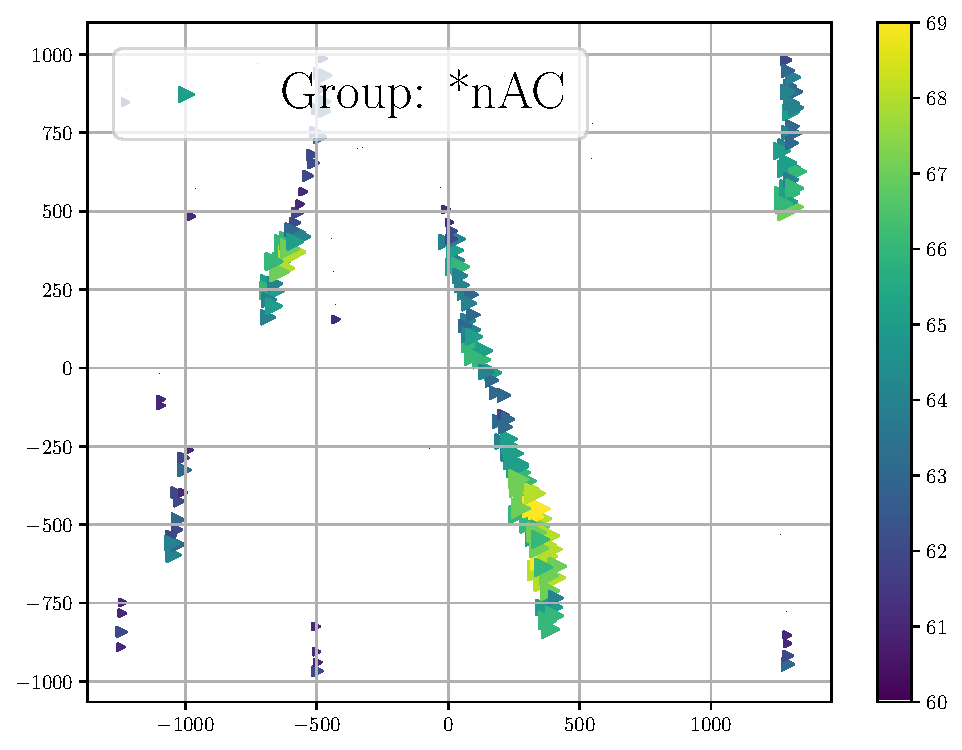
\includegraphics[width=1\textwidth]{Img/chapter10/PI-Class-group-sample5.pdf}
         \caption{Group行为对应合作关系描述示意图}
         \label{group-sample5-coh1}
     \end{subfigure}
     \hfill
     \begin{subfigure}[b]{.45\textwidth}
         \centering
         \includegraphics[width=1\textwidth]{Img/chapter10/Class-align-sample4.pdf}
         \caption{无人机集群Align行为示意图}
         \label{align-sample5-coh}
     \end{subfigure}
     \hfill
     \begin{subfigure}[b]{.45\textwidth}
         \centering
         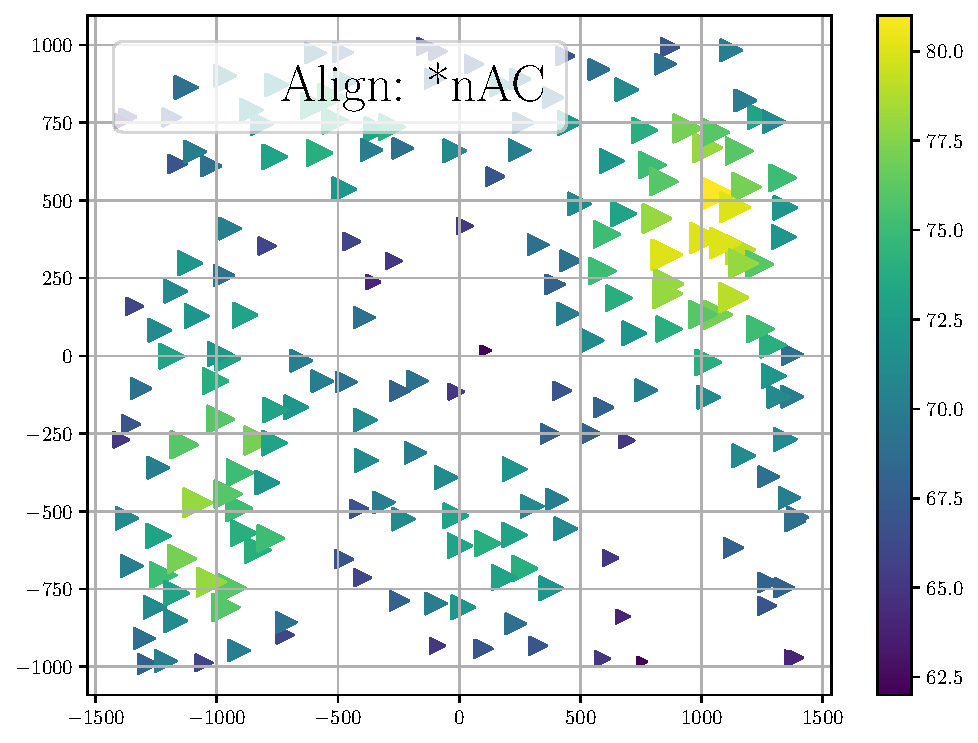
\includegraphics[width=1\textwidth]{Img/chapter10/PI-Class-align-sample4.pdf}
         \caption{Align行为对应合作关系描述示意图}
         \label{align-sample5-coh1}
     \end{subfigure}          
\caption{智能体合作关系的整体描述示意图}
\label{fig:nAC-demon}
\end{figure}

这就可以给一种启示, 如果将这类合作特权信息加入模型, 会不会能够增加学习的收敛速率。类似的结果也在 Align行为中得以展现, 图 \ref{align-sample5-coh} 的展示的是Align行为, 其对应的特权信息{Align: *nAC}为图\ref{align-sample5-coh1}。 从图中可以直观地看到类似的结果, 即对于Align行为, 特权信息{Align: *nAC}在智能体聚集的区域取值较高, 在智能体分散的区域取值较低。 因此, 希望这种对智能体直观的整体描述能够加速集群行为识别的收敛速率。

另外, 还提出另一种整体性描述智能体的特权信息。 将处在Separation向量半径内的智能体数目视作是竞争描述。 从介绍无人机集群行为数据集的描述中可知, Separation向量刻画的是智能体彼此之间处于分离状态的向量, 因此, 在Separation向量半径内的智能体数目直观上可以视为是一种竞争关系的尺度。图\ref{fig:nS-demon} 展示两种集群行为下所对应的竞争关系。 图 \ref{group-sample5-jz} 展示的是Group行为, 此时其对应的特权信息是图\ref{group-sample5-jz1}。 特权信息{Group:*nS}图中采用热力图标示{nS}数目的大小区别, 从图中可以看到, 智能体聚集的部分其特权信息{Group: *nS}的取值较高, 智能体分散的部分其特权信息{Group: *nS}的取值较低。 

%
%\begin{figure}
%\centering
%\includegraphics[width=.4\textwidth]{Class-group-sample5.pdf}
%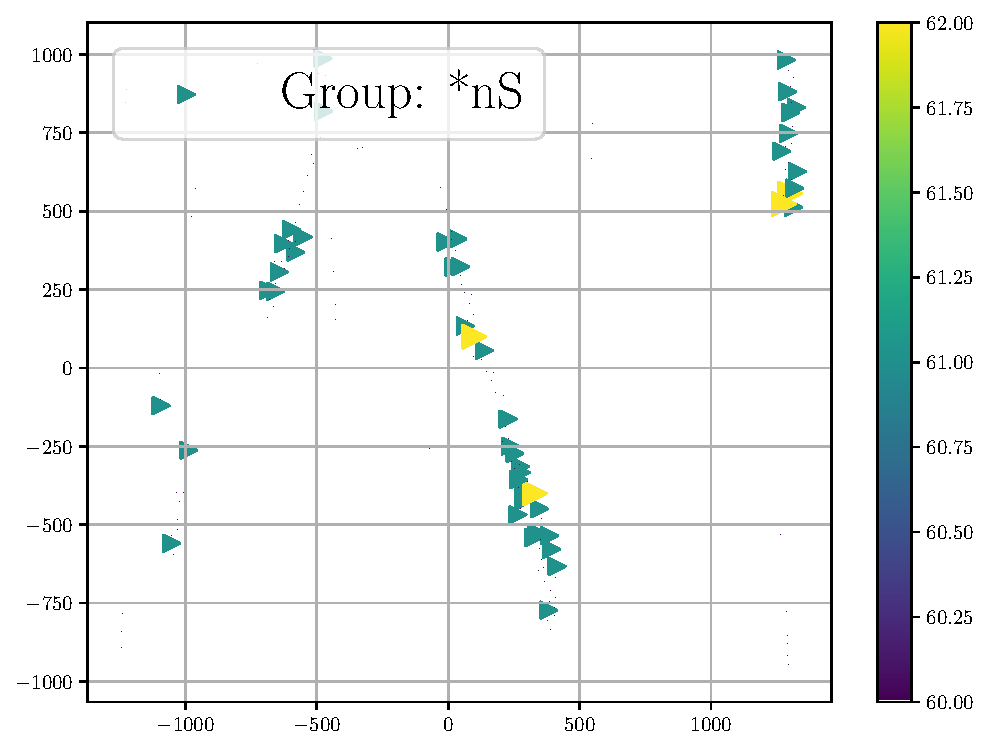
\includegraphics[width=.4\textwidth]{S-PI-Class-group-sample5.pdf}
%\includegraphics[width=.4\textwidth]{Class-align-sample4.pdf}
%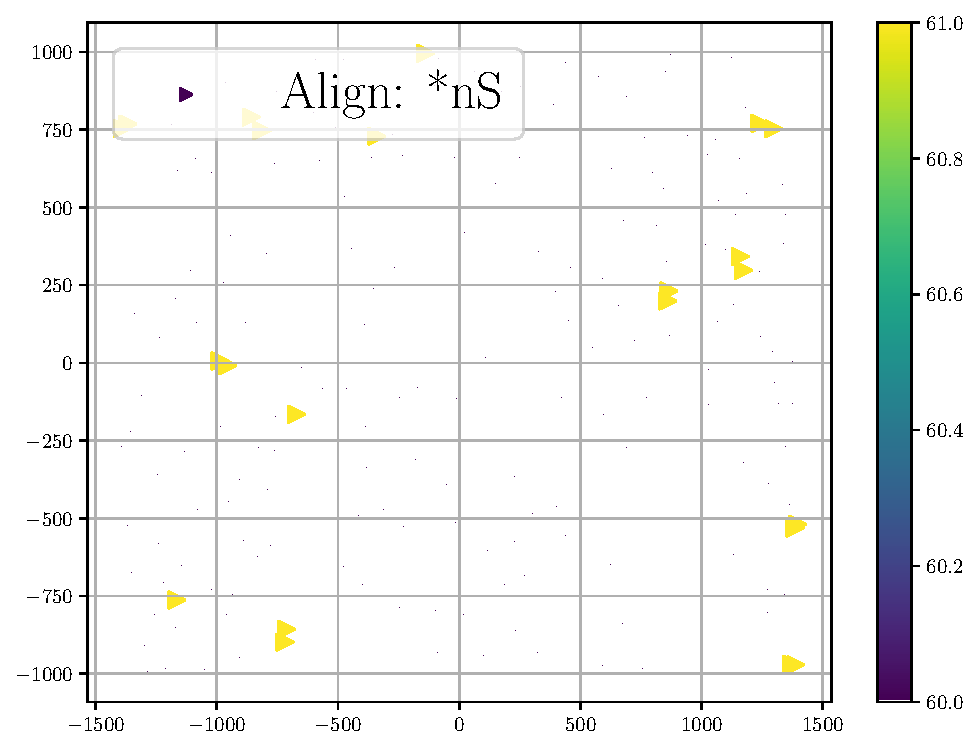
\includegraphics[width=.4\textwidth]{S-PI-Class-align-sample4.pdf}
%\caption{智能体竞争关系的整体描述示意图}
%\label{fig:nS-demon}
%\end{figure}

\begin{figure}
     \centering
     \begin{subfigure}[b]{.45\textwidth}
         \centering
         \includegraphics[width=1\textwidth]{Class-group-sample5.pdf}   
         \caption{无人机集群Group行为示意图}
         \label{group-sample5-jz}
     \end{subfigure}
     \hfill
     \begin{subfigure}[b]{.45\textwidth}
         \centering
         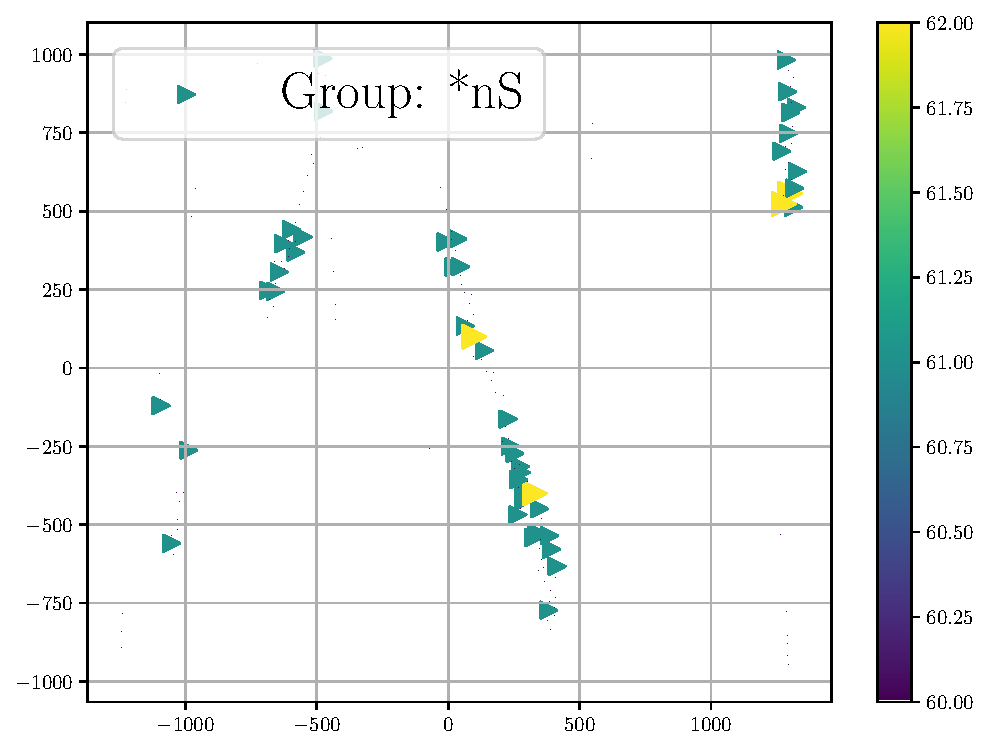
\includegraphics[width=1\textwidth]{S-PI-Class-group-sample5.pdf}
         \caption{Group行为对应竞争关系描述示意图}
         \label{group-sample5-jz1}
     \end{subfigure}
     \hfill
     \begin{subfigure}[b]{.45\textwidth}
         \centering
         \includegraphics[width=1\textwidth]{Class-align-sample4.pdf}
         \caption{无人机集群Align行为示意图}
         \label{align-sample5-jz}
     \end{subfigure}
     \hfill
     \begin{subfigure}[b]{.45\textwidth}
         \centering
         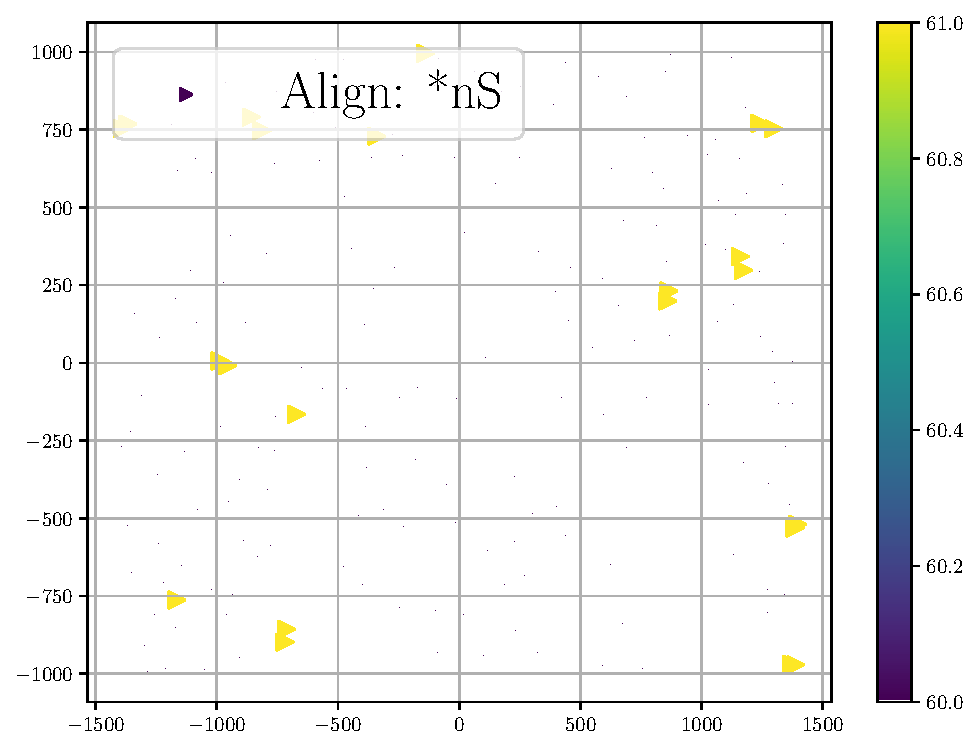
\includegraphics[width=1\textwidth]{S-PI-Class-align-sample4.pdf}
         \caption{Align行为对应竞争关系描述示意图}
         \label{align-sample5-jz1}
     \end{subfigure}          
\caption{智能体竞争关系的整体描述示意图}
\label{fig:nS-demon}
\end{figure}

同样地, 如果将这类反映智能体“竞争激烈”的特权信息加入模型, 会不会能够增加学习的收敛速率。 类似的结果也在 Align行为中得以展现, 图 \ref{align-sample5-jz} 展示的是Align行为, 其对应的特权信息{Align: *nS}为图\ref{align-sample5-jz1} 所示。整体上而言, 特权信息{Align: *nS}在智能体聚集的区域取值较高, 在智能体分散的区域取值较低。 这些取值高低的分布可以朴素地理解为智能体之间“竞争”的激烈程度的度量。因此, 希望这种对智能体直观的竞争描述也能够加速集群行为识别的收敛速率。

对于特权学习建模, 考虑两种建模方法, 
\begin{enumerate}
\item[1.] 一般通用LUPI算法 (LUPI-X*): 在这种模型中, 特权空间直接由核函数 $K^{*}(x_{i}^{*},x_{j}^{*})$定义。
\item[2.] 特定具体LUPI算法 (LUPI-d): 在这种模型中, 特权空间是由具体的一维 $d$-空间所定义的, 此$d$-空间是由SVMs按照下列步骤实施的, 即
\begin{enumerate}
\item[(1)] 首先, 给定下列数据对
\begin{align}
(x_{1}^{*}, y_{1}), \ldots, (x_{l}^{*},y_{l}).
\end{align}
考虑在空间 $X^{*}$中寻找一个决策规则, 然后提取此问题的得分函数 $\hat{y}_{i}$。
\item[(2)] 使用在空间$X^{*}$中的得分函数来定义下列偏差值 $d_{i} = 1-y_{i}\hat{y}_{i}$。
\item[(3)] 使用下列三元组构建LUPI模型
\begin{align}
(x_{1}, d_{1}, y_{1}), \ldots, (x_{l}, d_{1}, y_{l}).
\end{align}
\end{enumerate} 
\end{enumerate}

在下一章节将展示一般通用LUPI算法和特定具体LUPI算法在集群行为数据集上的结果。

\section{整体描述作为特权信息加速分类算法收敛研究}

本节介绍两种针对无人机集群行为的整体描述作为特权信息, 加速LUPI算法收敛。第一种整体描述信息提供了针对无人机集群的合作描述; 第二种整体描述信息提供了针对无人机集群的竞争描述。

\subsection{无人机集群的合作描述作为特权信息}
本节针对合作描述作为特权信息的LUPI方案设计展开研究。提出诸智能体之间彼此如何“合作”的整体描述作为特权信息来验证LUPI方法的有效性和优势。 按照集群行为数据的原始顺序将数据切分为两部分: 使用前100个数据作为训练集, 后面10000个数据用于测试集, 重复试验20次取平均值。 这里需要专门指出, 确实是采用小量样本训练而测试大样本。 

考虑四种不同的机器学习算法进行对比, 分别是经典SVMs算法, 神经网络算法, LUPI-X*算法和LUPI-d算法。四种算法都采取默认参数, 即在SVMs中采用RBF核函数, 容量因子C=1; 在神经网络算法中采用默认参数, LUPI中决策空间采用RBF核函数, 特权空间采用线性核函数。 这四种算法分别在三种集群行为数据集上训练。 表\ref{tab:PI-nAC-LUPI-X}和表\ref{tab:PI-nAC-LUPI-d}分别列出了合作关系作为特权信息的LUPI-X*方法和LUPI-d方法分类准确度对比表。

具体而言, 对于表\ref{tab:PI-nAC-LUPI-X}中的Align数据集, 标准的SVMs算法和神经网络算法分别获得 74.54\% 和 48.57\% 的分类准确度, LUPI-X*方法将之提升至 82.31\%, 提升幅度分别为10.42\%和69.47\%; 对于Flock数据集, 标准的SVMs算法和神经网络算法分别获得 50.59\% 和 59.26\% 的分类准确度, LUPI-X*方法将之提升至 60.65\%, 提升幅度分别为19.04\%和2.35\%; 对于Group数据集, 标准的SVMs算法和神经网络算法分别获得 59.24\% 和 44.36\% 的分类准确度, LUPI-X*方法将之提升至 64.45\%, 提升幅度分别为9.79\%和45.29\%。

对于LUPI-d算法, 如表\ref{tab:PI-nAC-LUPI-d}结果所示, 对于Align数据集, 标准的SVMs算法和神经网络算法分别获得 74.54\% 和 48.57\% 的分类准确度, LUPI-d方法将之提升至 82.31\%, 提升幅度分别为10.42\%和69.47\%; 对于Flock数据集, 标准的SVMs算法和神经网络算法分别获得 50.59\% 和 59.26\% 的分类准确度, LUPI-d方法将之提升至 66.79\%, 提升幅度分别为31.09\%和12.71\%; 对于Group数据集, 标准的SVMs算法和神经网络算法分别获得 59.24\% 和 44.36\% 的分类准确度, LUPI-d方法将之提升至 73.55\%, 提升幅度分别为24.16\%和65.80\%。

\begin{table}[]
\centering
\caption{合作关系作为特权信息的LUPI-X*方法分类准确度对比表}
\label{tab:PI-nAC-LUPI-X}
\begin{tabular}{cccccc}
\hline
      & SVMs   & \begin{tabular}[c]{@{}c@{}}神经 \\ 网络\end{tabular} & LUPI-X* & \begin{tabular}[c]{@{}c@{}}LUPI-X*较SVMs\\ 提升百分比\end{tabular} & \begin{tabular}[c]{@{}c@{}}LUPI-X*较NN\\ 提升百分比\end{tabular} \\ \hline
Align & 74.54 & 48.57                                                      & \textbf{82.31}   & 10.42\%                                                     & 69.47\%                                                    \\
Flock & 50.95 & 59.26                                                      & \textbf{60.65}   & 19.04\%                                                     & 2.35\%                                                     \\
Group & 59.24 & 44.36                                                      & \textbf{64.45}   & 9.79\%                                                      & 45.29\%                                                    \\ \hline
\end{tabular}%
\end{table}

% Please add the following required packages to your document preamble:
% \usepackage{graphicx}
\begin{table}[]
\centering
\caption{合作关系作为特权信息的LUPI-d方法分类准确度对比表}
\label{tab:PI-nAC-LUPI-d}
\begin{tabular}{cccccc}
\hline
      & SVMs   & \begin{tabular}[c]{@{}c@{}}神经 \\ 网络\end{tabular} & LUPI-d & \begin{tabular}[c]{@{}c@{}}LUPI-d较SVMs\\ 提升百分比\end{tabular} & \begin{tabular}[c]{@{}c@{}}LUPI-d较NN\\ 提升百分比\end{tabular} \\ \hline
Align & 74.54 & 48.57                                                      & \textbf{82.31}  & 10.42\%                                                    & 69.47\%                                                   \\
Flock & 50.95 & 59.26                                                      & \textbf{66.79}  & 31.09\%                                                    & 12.71\%                                                   \\
Group & 59.24 & 44.36                                                      & \textbf{73.55}  & 24.16\%                                                    & 65.80\%                                                   \\ \hline
\end{tabular}%
\end{table}


以上结果表明, 通过考量在训练阶段可用但是无法在测试阶段采用的有关无人机集群整体合作关系的描述, 基于LUPI方法能够提升模型的学习推广能力。 同时这些试验表明, 特定具体LUPI算法(即LUPI-d方法)的学习推广能力最优, 这也能够支持\citet{Vapnik-similary-2015,vapnik2015}提出的知识转换的结果。

众所周知, 无人机集群研究中智能体数目会影响智能体彼此之间的合作关系。直观而言, 智能体数目越多, 合作关系越突出, LUPI算法中引进的特权信息对模型的贡献度应该越明显。 因此在不同的算法下考察智能体数目对分类准确度的影响, 对比智能体数目从10至100之间, 不同算法的预测准确度。

图 \ref{fig:agents-accuracy} 给出SVMs算法、神经网络算法和LUPI-d算法三种算法的预测结果。 从图中可以看到标准SVMs算法作为基准算法, 其预测性能表现保持稳定。对于神经网络算法采用默认全连接参数, 因为没有进行参数优化, 所以全连接神经网络算法的预测表现并不稳定。考虑整体描述信息的LUPI算法随着智能体数目增加到一定规模后, 其预测能力稳步提升, 并且整体上均由于其他两种算法。 

\begin{figure}
\centering
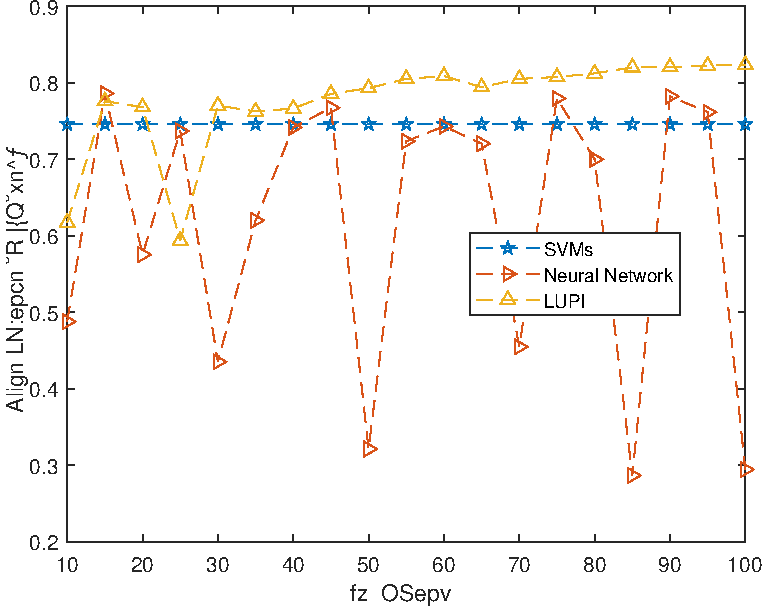
\includegraphics[width=.7\textwidth]{Img/chapter10/align-agent-PI1.pdf}
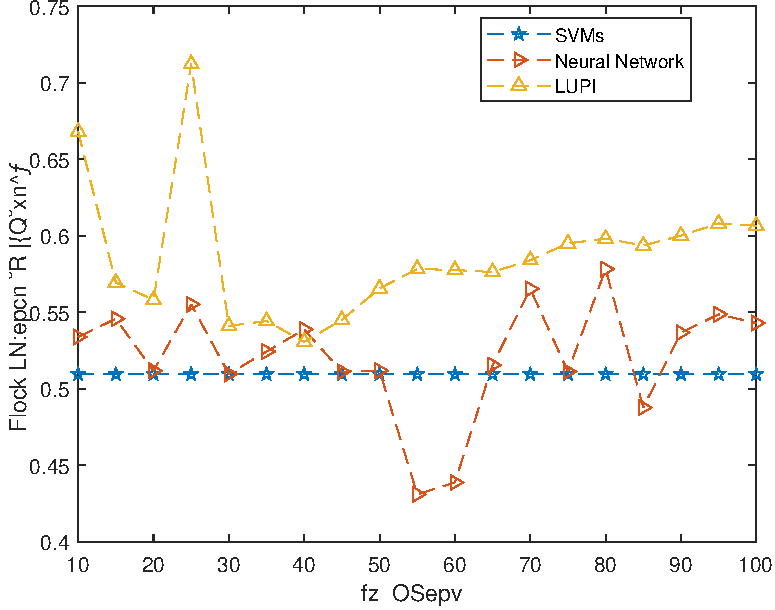
\includegraphics[width=.7\textwidth]{Img/chapter10/flock-agent-PI1.pdf}
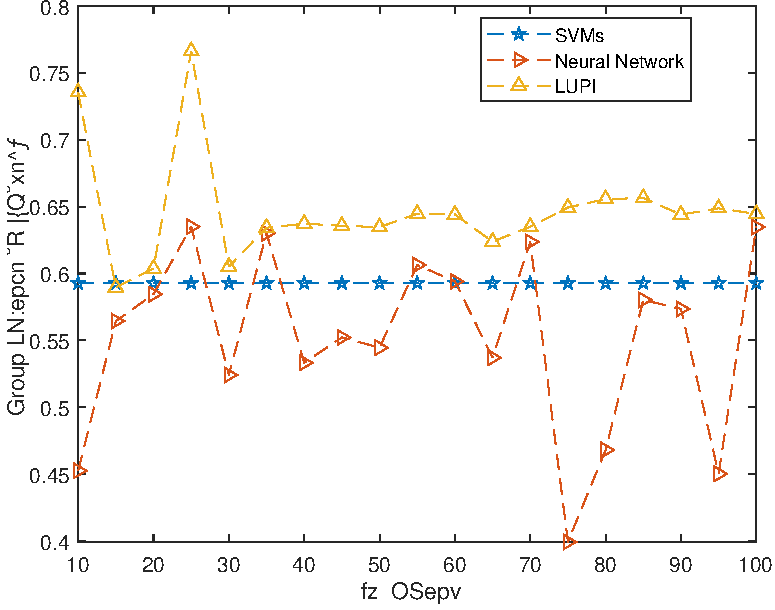
\includegraphics[width=.7\textwidth]{Img/chapter10/group-agent-PI1.pdf}
\caption{合作关系作为特权信息的LUPI方法分类准确度比较}
\label{fig:agents-accuracy}
\end{figure}

具体而言, 对于Align数据集 (图\ref{fig:agents-accuracy}上图)SVMs算法的预测准确率集中在0.7454; 神经网络算法受集群智能体个数的影响波动比较大, 并且总体而言其学习推广能力相较于SVMs算法和LUPI算法都较差; LUPI算法在当智能体数目小于30时, 学习推广能力波动较大, 但是当智能体数目大于30之后, LUPI算法的学习推广能力明显优于SVMs算法和神经网络算法。对于Flock数据集 (图\ref{fig:agents-accuracy}中图), SVMs算法预测性能并不会随着智能体数目的变化发生很大的波动, 而神经网络算法同样表现出比较大的波动, LUPI算法则明显优于另外两种算法。 最后, 相同的结果也适用于Group数据集 (图\ref{fig:agents-accuracy}下图), 即SVMs算法能够得到相对稳定的结果, 神经网络算法受智能体数目增加的影响会产生较大的波动, 并且大多数情形下其学习推广能力都表现的不尽人意 (因为都采取的是默认参数, 此时的神经网络未经过参数寻优), 而LUPI算法则随着智能体数目的增加, 其学习推广能力会稳定地优于另两种现代机器学习算法。


\subsection{无人机集群的竞争描述作为特权信息}
对于仿生集群行为分类问题, 与之前所述的合作关系类似, 考虑智能体彼此之间的竞争关系。 对于仿生集群行为, Separation向量描述智能体彼此之间的分离关系, 因此直观上而言, 可以借用每个智能体处在Separation向量半径内的数目来刻画智能体彼此之间的“竞争关系”。还是按照数据集原初顺序将集群数据集分为训练集和测试集并且择使用150个训练样本预测后面10000个数据。

表 \ref{tab:sample-error-LUPI-X} 和表 \ref{tab:sample-error-LUPI-d} 列出将竞争描述作为特权信息的LUPI方法在此实验下利用四种学习算法的分类准确率, 这两个表中所得结果是相同的。 其中, 四种算法都采取默认参数, 即在SVMs中采用RBF核函数, 容量因子C=1; 在神经网络算法中采用默认参数, LUPI中决策空间采用RBF核函数, 特权空间采用线性核函数。 这四种算法分别在三种集群行为数据集上训练, 从表\ref{tab:sample-error-LUPI-X} 和表 \ref{tab:sample-error-LUPI-d}可以看到, 对于Align行为数据集, LUPI-X*算法和LUPI-d算法比常规SVMs算法提升13.70\%, 而对神经网络算法则提升高达143.96\%; 对于Flock行为数据集, LUPI-X*算法和LUPI-d算法比常规SVMs算法提升20.63\%, 而对神经网络算法则提升高达68.75\%; 对于Group行为数据集, LUPI-X*算法和LUPI-d算法比常规SVMs算法提升11.14\%, 但对神经网络算法则没有提升, 但是两者预测效果相差不大。


\begin{table}[]
\centering
\caption{竞争关系作为特权信息的LUPI-X*方法分类准确度对比表}
\label{tab:sample-error-LUPI-X}
\begin{tabular}{cccccc}
\hline
      & SVMs   & \begin{tabular}[c]{@{}c@{}}神经 \\ 网络\end{tabular} & LUPI-X* & \begin{tabular}[c]{@{}c@{}}LUPI-X*较SVMs\\ 提升百分比\end{tabular} & \begin{tabular}[c]{@{}c@{}}LUPI-X*较NN\\ 提升百分比\end{tabular} \\ \hline
Align & 74.54 & 37.74                                                      & \textbf{84.75}   & 13.70\%                                                     & 143.96\%                                                   \\
Flock & 50.85 & 36.35                                                      & \textbf{61.34}   & 20.63\%                                                     & 68.75\%                                                    \\
Group & 59.27 & \textbf{66.41}                                                      & 65.87   & 11.14\%                                                     & -0.81\%                                                    \\ \hline
\end{tabular}%
\end{table}

\begin{table}[]
\centering
\caption{竞争关系作为特权信息的LUPI-d方法分类准确度对比表}
\label{tab:sample-error-LUPI-d}
\begin{tabular}{cccccc}
\hline
      & SVMs   & \begin{tabular}[c]{@{}c@{}}神经 \\ 网络\end{tabular} & LUPI-d & \begin{tabular}[c]{@{}c@{}}LUPI-d较SVMs\\ 提升百分比\end{tabular} & \begin{tabular}[c]{@{}c@{}}LUPI-d较NN\\ 提升百分比\end{tabular} \\ \hline
Align & 74.54 & 37.74                                                      & \textbf{84.75}   & 13.70\%                                                     & 143.96\%                                                   \\
Flock & 50.85 & 36.35                                                      & \textbf{61.34}   & 20.63\%                                                     & 68.75\%                                                    \\
Group & 59.27 & \textbf{66.41}                                                      & 65.87   & 11.14\%                                                     & -0.81\%                                                    \\ \hline
\end{tabular}%
\end{table}


具体而言, 对于Align数据集, LUPI系列算法比标准SVMs算法和神经网络算法都优异; 标准的SVMs算法和神经网络算法分别获得 74.54\% 和 37.74\% 的分类准确度, 而LUPI方法将之提升至 84.75 \%; 对于Flock数据集, 标准的SVMs算法和神经网络算法分别获得 50.85\% 和 36.35\% 的分类准确度, LUPI系列方法将之提升至 61.34 \%分类准确度; 而对于Group数据集, 标准的SVMs算法和神经网络算法分别获得 59.27\% 和 66.41\% 的分类准确度, LUPI系列方法分别获得 65.87\% 的分类准确度, 稍微低于最优的神经网络算法。 这些结果都表明, 通过考量在训练阶段可用但是无法在测试阶段采用的有关无人机集群的整体竞争关系描述, LUPI方法能够提升模型的学习推广能力。 

同时, 讨论训练样本数目与收敛速率的关系。直观上而言, 随着样本数目增多算法更容易收敛。而根据VC理论可知LUPI算法有可能实现小样本下高精度预测, 即LUPI算法有可能不需要太多样本就可以实现高精度预测。因此, 考察随着样本数目的增加各个模型错误分类的变化关系。 图 \ref{fig:sample-error} 展示针对三种集群行为数据集, 当训练样本量从50增加至150时, 三种机器学习分类错误率的变化情况。 从图中可以看到, 总体而言LUPI方法能够保持最佳的学习推广能力, 其受样本量增加的影响比较小, 基本能够保持稳定的分类错误率, 特别是在小量样本下仍然能够获得最低的错误分类。 

\begin{figure}
\centering
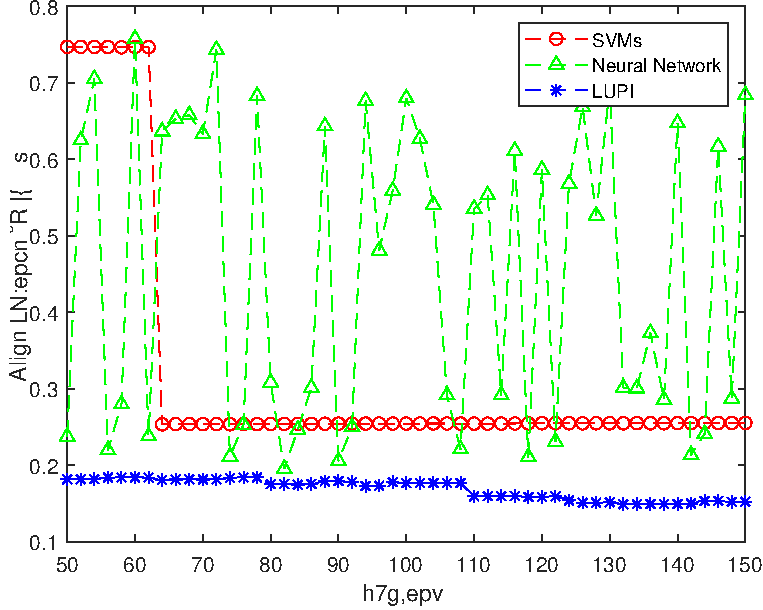
\includegraphics[width=.7\textwidth]{Img/chapter10/align-sample-PI2.pdf}
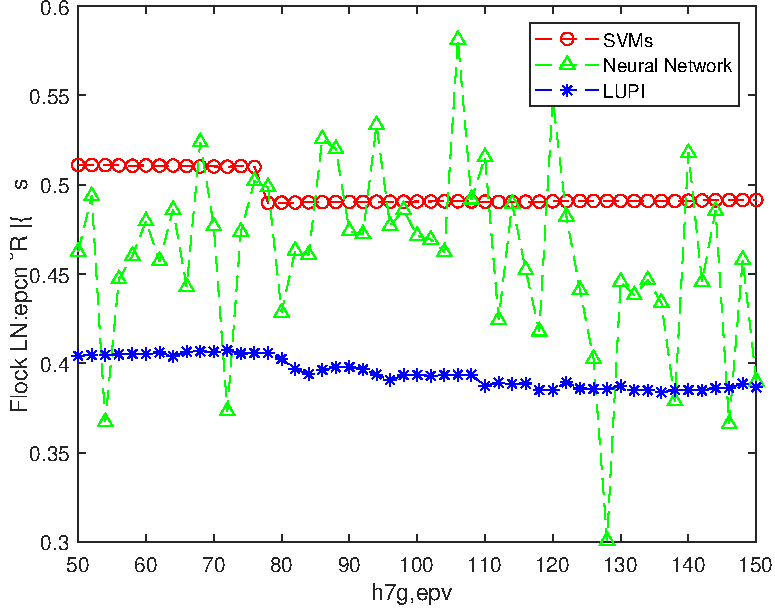
\includegraphics[width=.7\textwidth]{Img/chapter10/flock-sample-PI2.pdf}
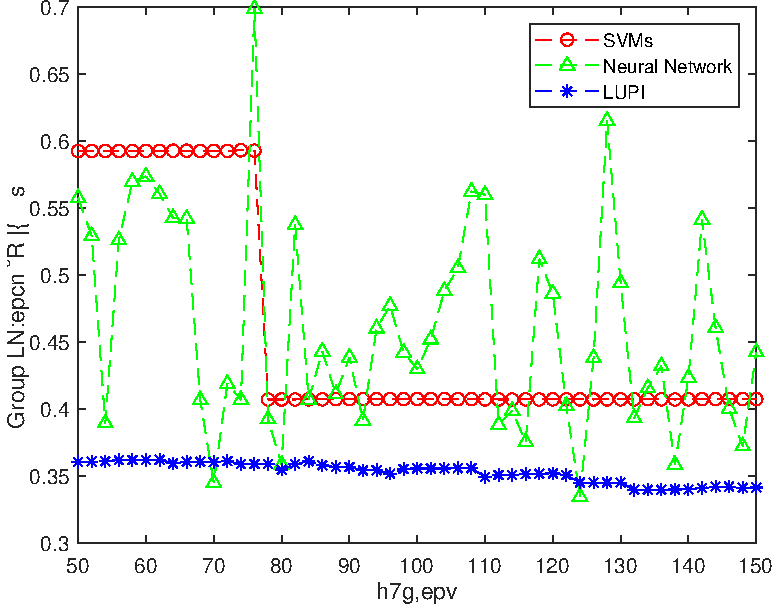
\includegraphics[width=.7\textwidth]{Img/chapter10/group-sample-PI2.pdf}
\caption{竞争关系作为特权信息的LUPI方法分类错误率比较}
\label{fig:sample-error}
\end{figure}


具体而言, 对于Align数据集 (图\ref{fig:sample-error}上图), 当样本小于60时, SVMs方法表现出最低的推广泛化能力, 其对应的分类错误率最高; 当样本数目大于60后, SVMs方法和LUPI方法预测效果趋于稳定, 并且LUPI方法的预测效果比SVMs方法要优异。 但是对于神经网络算法, 由于并没有进行网络参数优化, 所以导致神经网络算法的预测性能受训练样本数目改变的影响较大。 对于Flock数据集(图\ref{fig:sample-error}中图)和Group数据集 (图\ref{fig:sample-error}下图), LUPI算法也依然保持稳健且优异的预测能力, 另两种算法的表现与Align数据集保持类似的结果。 

这样的结果也符合的预期, 正如VC理论所指明的, 通过引进特权信息, LUPI算法确实可以加速学习模型的收敛速率 (在这三个数据集上, 完全可以只采用50个样本就可以达到比标准SVMs算法、神经网络算法更好的预测效果)。 这样的结果是不奇怪的, 因为借助LUPI算法能够对集群行为提供整体的描述, 这样就使得学习算法能够加速收敛速率。

  
\section{本章小结}
\label{sec:discuss}
本节为无人机集群行为分类提供一种使用特权信息学习(Learning Using Privileged Information, LUPI)的新方法, 这种学习方法通过融合在训练阶段可用但是在测试阶段不可用的信息(此信息称为“特权信息”)来加速学习算法的收敛速度。主要结论总结如下:
\begin{enumerate}
\item 研究针对无人机集群行为整体描述的合作关系作为特权信息时LUPI算法的效果。研究结果表明, LUPI方法能够显著提升算法预测精度, 在三种无人机集群行为数据集上较基准SVMs算法提升分别为10.42\%, 31.09\% 和 24.16\%;
\item 研究针对无人机集群行为整体描述的竞争关系作为特权信息时LUPI算法的效果。研究结果表明, LUPI方法大都能够提升算法预测精度, 在三种无人机集群行为数据集上较基准SVMs算法提升分别为13.70\%, 20.63\% 和 11.14\%;
\item 比较智能体数目与无人机集群合作关系的影响, 以及无人机集群训练样本数目与LUPI算法收敛速度的影响。研究结果表明, 采用LUPI算法能够提升学习算法的收敛速度, 实现在无人机集群行为分类任务中小样本高精度预测的目标。
\end{enumerate}
